%\{ {\it  sp1d\_ch3\_2.tex} \}

\subsubsection {High order Polynomial Solution and Its Convergence}

In this section we construct a polynomial $P_n$ of order $n$ defined on $[0,1]$, which satisfies the following.
\begin{eqnarray}
\label{pois_scrv}
    P_n(0) = 0, &P_n(1) = 1 \\
    \frac{d^k}{dx^k}P_n(0) = 0, &\frac{d^k}{dx^k}P_n(1) = 0
\end{eqnarray}
for all $k = 1, \cdots, n-2$. \\
For each $n$, we obtain polynomial $P_n$ by solving a system of
linear equations that determines the set of coefficients of $P_n$.
We use the spectral polynomial solver to approximate the second
derivative $Q_{n-2}$ of $P_n$.

\begin{figure}[h]
    \begin{center}
    \epsfig{file = Doc-Report_Fwd2D/figs_dn/ScrvH5_A.eps, width = 5cm}
    \epsfig{file = Doc-Report_Fwd2D/figs_dn/ScrvH5_N.eps, width = 5cm}
    \caption{\label{scrvsol}Example of curve that satisfies conditions (\ref{pois_scrv}) with polynomial order $n=7, 9, 12, 14, 15$. The error is $2.9239e-8$}
    \end{center}
\end{figure}

We investigate the convergences by the h-type, p-type extension of
trial functions below.

\begin{problem}
Consider the following differential equation for $u(x)$ such that
\begin{equation}
\label{poi_poly}
-r^2 \frac{\partial}{\partial r} (\sigma \frac{\partial}{\partial r}u) - r \sigma \frac{\partial}{\partial r}u - \sigma \frac{\partial^2}{\partial \theta^2}u = e^{-(r-1)^2}\{P_n(r) + (2r^2(r-1)-r)P_n'(r) - r^2 P_n''(r)\} \cos \theta,
\end{equation}
for all $r$ in $[0.1, 1.1]$ with $\sigma(r) = e^{-(r-1)^2}$.

The exact solution is known to be:
\begin{equation}
u(r, \theta) = P_n(r) \cos \theta
\end{equation}
where $r$ in $[0.1, 1.1]$ and $\theta$ in $[0, 2\pi]$.
\end{problem}

\begin{figure}[h]
\begin{center}
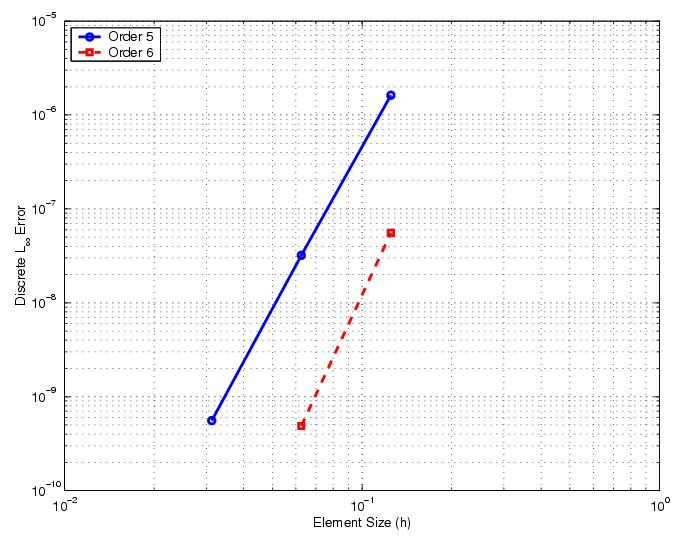
\epsfig{file = Doc-Report_Fwd2D/figs_dn/ScrvHconv.eps, width =
8.3cm} 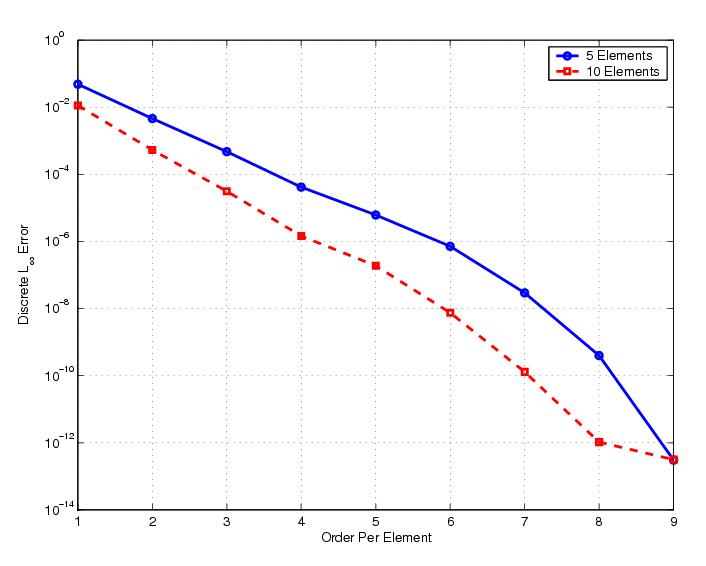
\epsfig{file = Doc-Report_Fwd2D/figs_dn/ScrvPconv.eps,
width = 8.3cm} \caption{\label{ScrvconvDN} (Left) Convergence with
respect to discrete $L^{\infty}$ norm as a function of size of
elements. This test is performed using the h-type extension with
fixed polynomials of order 3, 4, and 5 respectively. Error on the
Log-Log axis demonstrates the algebraic convergence of the h-type
extension. (Right) Convergence w.r.t. $L^{\infty}$ norm as a
function of size of polynomial order in semi-Log plot. It shows
the exponential convergence of p-type extension for smooth
solutions. The two tests are performed for p-type extension with
element lengths of $0.2$ and $0.1$. }
\end{center}
\end{figure}

\begin{table}[h]
\centering \caption{\label{hconv2t} This table shows the
convergence of h-type resolution control done above Figure
(\ref{ScrvconvDN}). We can see the slopes of each order $P$ is
$P+1$ }
\begin{tabular}{|c|c|c|} \hline
    Polynomial order&Error($L^{\infty}$)&Slope   \\ \hline \hline
    5&$8.5305e-012$ &$5.7556$ \\ \hline
    6&$4.7180e-012$ &$6.8332$ \\ \hline
\end{tabular}
\hspace{.5in}
\begin{tabular}{|c|c|} \hline
    {Element Size}&Error($L^{\infty}$) \\ \hline \hline
    0.2&$9.0616e-13$  \\ \hline
    0.1&$9.4747e-13$ \\ \hline
\end{tabular}
\end{table}
